\section{Manipulador Robótico}
\label{sec:manipulador_robotico}

O manipulador robótico (MR) é responsável pelas operações de captura e acoplamento durante a fase final da missão de RVD/B.
Tratando-se de ambiente de microgravidade, a sensação da ausência da força peso ($\vec P = m \vec g$) elimina as forças gravitacionais locais, mas não os efeitos de reação gerados pela movimentação do MR.
Essas movimentações alteram a atitude e a inércia equivalente da base da espaçonave.
A interação dinâmica entre a base e o MR exige uma formulação integrada para representar o comportamento do conjunto.

O desempenho do MR está condicionado por restrições cinemáticas e estruturais, como os limites de junta, as dimensões dos elos, a capacidade de torque e a velocidade dos atuadores.
As limitações definem o espaço de trabalho (\emph{workspace}) e impõem ligações entre alcance, precisão e estabilidade do sistema.

A seguir, é apresentado o propósito do MR no contexto da missão, definindo suas funções, movimentos requeridos e graus de liberdade necessários.

\subsection{Propósito e Arquitetura}
\label{sec:proposito_arquitetura}

O manipulador robótico realiza tarefas de captura, manipulação e acoplamento durante as operações de RVD/B.
Após a aproximação da espaçonave visitante, o MR atua na fase final de acoplamento, realizando movimentos de alinhamento e fixação entre o efetuador $\{E\}$ e a porta de acoplamento do alvo.
Nessa etapa, o controle orbital é substituído por uma dinâmica de contato, em que o manipulador e a base passam a interagir mecanicamente por meio das forças de reação internas.

Por estar em um ambiente de microgravidade, a conservação do momento angular total do sistema acopla o movimento da base e o do manipulador, portanto, cada movimento das juntas do MR gera torques de reação que afetam a atitude da base, exigindo que o controle de orientação compense essas alterações.
A compensação é implementada por estratégia de controle acoplado, as quais a cinemática e a dinâmica do MR são incorporadas às leis de controle de atitude.

A configuração adotada para o MR é do tipo 4R1P, sendo quatro juntas revolutas que realizam o posicionamento e orientação da ferramenta, e uma junta prismática, que fornece extensão linear ao efetuador.
Além disso, o projeto do MR leva em conta as restrições físicas e operacionais, como os limites de curso das juntas, capacidade máxima de torque e a velocidade dos atuadores.

\subsection{Atribuição dos referenciais e das variáveis generalizadas}
\label{sec:referenciais_variaveisGeneralizadas}

Foi utilizado referenciais e variáveis generalizadas para realizar a modelagem cinemática e dinâmica do manipulador robótico para então descrever o movimento do MR.
Nesta pesquisa, a convenção de clássica de Denavit--Hartenberg (DH) é utilizada para fixar os referenciais aos elos e representar a transformação geométrica entre eles.

\begin{figure}[ht]
\centering
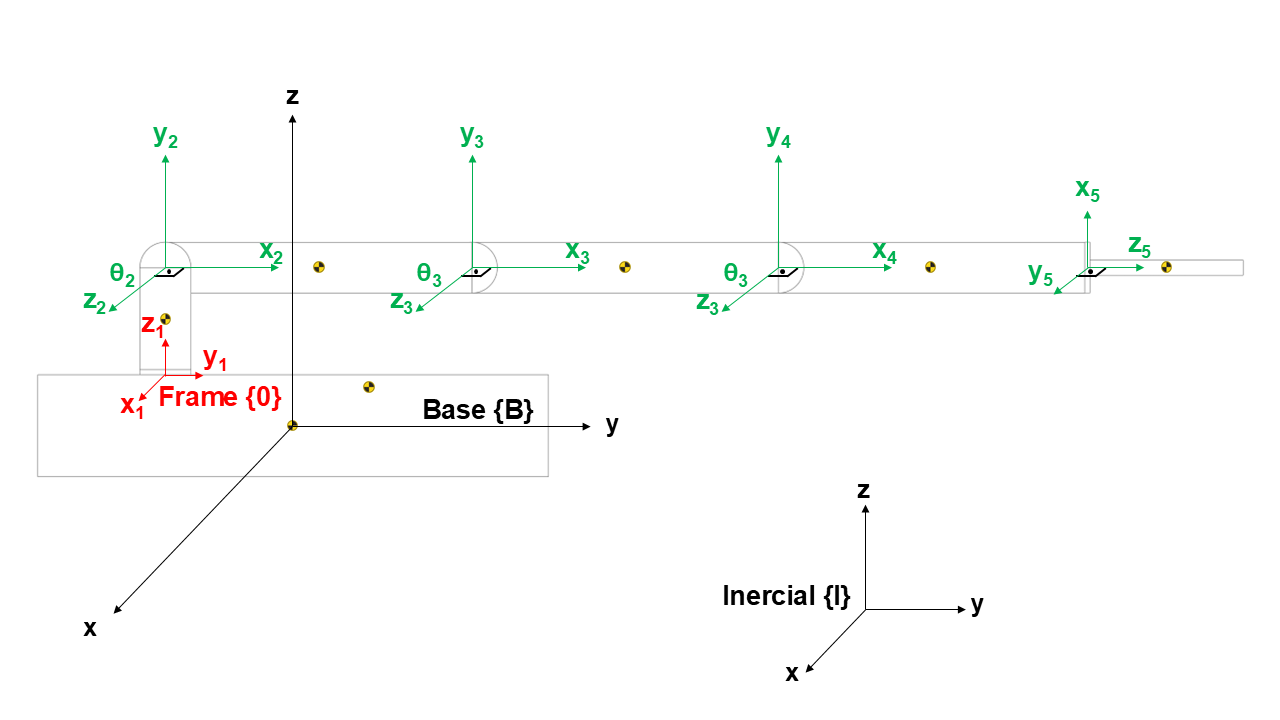
\includegraphics[width=1\textwidth]{2 Formulacao do problema/Imagens/MR Coordenadas locais.png}
\caption{Referencial local do Manipulado Robótico 4R1P acoplado à base.}
\label{fig:frames_MR}
\end{figure}

O sistema de coordenadas inercial $\{I\}$ é utilizado como referência absoluta, enquanto que o referencial da base $\{B\}$ tem sua origem no centro de massa da base e os seus eixos estão alinhados conforme a orientação do corpo, além disso, o referencial $\{0\}$ está na base do primeiro elo do MR.
Os referenciais locais $\{i\}$ ($i=1,\dots,5$) são fixados em cada elo do manipulador, conforme as atribuições de DH:

\begin{enumerate}[label=(\roman*)]
    \item o eixo $Z_i$ coincide com o eixo de rotação (ou de deslizamento) da junta $i$;
    \item o eixo $X_i$ é definido como perpendicular comum entre $Z_i$ e $Z_{i+1}$ e aponta de $Z_i$ para $Z_{i+1}$;
    \item o eixo $Y_i$ completa o sistema dextrogiro.
\end{enumerate}

A posição e a orientação de cada elo em relação ao anterior são expressas pela matriz de transformação homogênea
${}^{i-1}A_i$, expressa por:

\begin{equation}
\label{eq:transformacao_DH}
{}^{i-1} A_i =
\begin{bmatrix}
\cos\theta_i & -\sin\theta_i\cos\alpha_{i-1} & \sin\theta_i\sin\alpha_{i-1} & a_{i-1}\cos\theta_i \\[4pt]
\sin\theta_i & \cos\theta_i\cos\alpha_{i-1} & -\cos\theta_i\sin\alpha_{i-1} & a_{i-1}\sin\theta_i \\[4pt]
0 & \sin\alpha_{i-1} & \cos\alpha_{i-1} & d_i \\[4pt]
0 & 0 & 0 & 1
\end{bmatrix}.
\end{equation}

Faz-se o produto sucessivo dessa matriz para obter a transformação global entre a base e o efetuador $\{E\}$:

\begin{equation}
\label{eq:transformacao_total}
{}^{B} T_{E}
=
{}^{B} T_1\,
{}^{1} T_2\,
{}^{2} T_3\,
{}^{3} T_4\,
{}^{4} T_5,
\end{equation}

sendo que ${}^{B} T_{E}$ descreve a posição e a orientação do efetuador em relação à base.
O estado generalizado do sistema acoplado base--manipulador, é definido pelo o vetor:

\begin{equation}
\label{eq:vetor_q}
\vec{q} =
\begin{bmatrix}
\vec{r}_B \\[4pt]
\vec{\eta}_B \\[4pt]
\vec{\theta}
\end{bmatrix},
\end{equation}

onde:
\begin{itemize}
    \item $\vec{r}_B$ é a posição do centro de massa da base no referencial inercial $\{I\}$;
    \item $\vec{\eta}_B$ descreve a atitude da base e pode ser expressa tanto por ângulos de Euler como por um quaternion unitário $q_B$;
    \item $\vec{\theta} = [\theta_1,\theta_2,\theta_3,\theta_4,d_5]^T$ são as variáveis articulares do manipulador robótico 4R1P.
\end{itemize}

Para relacionar as velocidades lineares e as velocidades angulares dos elos consecutivos utiliza-se a equação diferencial das transformações homogêneas.
Seja ${}^{i-1} \vec{\omega}_i$ a velocidade angular do elo $i$ em relação ao elo anterior $i-1$, e seja ${}^{i-1}\,\vec{v}_i$ a velocidade linear do ponto de origem de $\{i\}$; então:

\begin{equation}
\label{eq:relacao_velocidades}
{}^{i} \vec{v}_i
=
{}^{i}R_{i-1} \left( {}^{i-1} \vec{v}_{i-1} + {}^{i-1} \vec{\omega}_{i-1} \times {}^{i-1} \vec{r}_{i-1,i} \right),
\end{equation}

onde ${}^{i}R_{i-1}$ é a matriz de rotação entre os referenciais e ${}^{i-1} \vec{r}_{i-1,i}$ é o vetor de posição do referencial $\{i\}$ em relação ao anterior $\{i-1\}$.
\subsection{Cinemática e relação de velocidades}
\label{sec:cinematica_velocidades}

Nesta subseção será estabelecida a relação cinemática entre a base $\{B\}$ e o efetuador $\{E\}$ do MR. Será evidenciado através do acoplamento por meio de um Jacobiano que inclui as velocidades generalizadas da base e das juntas. O referencial utilizado é o da base $\{B\}$.

A pose (orientação e posição) do efetuador é dada por \eqref{eq:transformacao_total}, enquanto que a posição do efetuador em relação à base $\{B\}$ é o vetor coluna de translação de \eqref{eq:transformacao_total}:

\begin{equation}
\label{eq:rBE}
{}^{B}\vec r_{BE} \;=\; \text{pos}\big({}^{B}T_{E}(\vec\theta)\big).
\end{equation}

Para definir as velocidades generalizadas da base $\{B\}$, faz-se:

\begin{equation}
\label{eq:nu_base}
\dot{\vec q}_B \;=\;
\begin{bmatrix}
{}^{B}\vec v_B \\[2pt]
{}^{B}\vec \omega_B
\end{bmatrix},
\qquad
\dot{\vec\theta} \;=\; [\,\dot\theta_1,\dot\theta_2,\dot\theta_3,\dot\theta_4,\dot d_5\,]^T.
\end{equation}

A velocidade espacial (twist) do efetuador $\{E\}$, também em relação à base $\{B\}$ é dado por:

\begin{equation}
\label{eq:twist_coupled}
\begin{bmatrix}
{}^{B}\vec v_E \\[2pt]
{}^{B}\vec \omega_E
\end{bmatrix}
\;=\;
J_B(\vec q)\,
\begin{bmatrix}
{}^{B}\vec v_B \\[2pt]
{}^{B}\vec \omega_B
\end{bmatrix}
\;+\;
J_m(\vec q)\,\dot{\vec\theta},
\end{equation}

onde $J_B$ é o Jacobiano que propaga a velocidade espacial da base até o efetuador; enquanto que $J_m$ é o Jacobiano geométrico do manipulador.

O termo $J_B$ decorre da cinemática de um corpo rígido:

\begin{equation}
\label{eq:JB}
J_B(\vec q)
\;=\;
\begin{bmatrix}
I_{3} & -\,[\,{}^{B}\vec r_{BE}\,]_{\times} \\
0_{3\times 3} & I_{3}
\end{bmatrix},
\end{equation}

de modo que:

\begin{equation}
\label{eq:vE_from_vB}
{}^{B}\vec v_E \;=\; {}^{B}\vec v_B \;+\; {}^{B}\vec \omega_B \times {}^{B}\vec r_{BE},
\qquad
{}^{B}\vec \omega_E \;=\; {}^{B}\vec \omega_B.
\end{equation}

O Jacobiano do manipulador é construído coluna a coluna, a partir dos eixos articulares em relação à base $\{B\}$.
Considerando ${}^{B}\hat z_i$ o eixo da junta $i$ e ${}^{B}\vec r_i$ a origem do referencial da junta $i$, ambos obtidos de ${}^{B}T_i$:

\begin{equation}
\label{eq:Jm_colunas}
J_m(\vec q) \;=\; \big[\, \mathcal{J}_1 \;\mathcal{J}_2 \;\mathcal{J}_3 \;\mathcal{J}_4 \;\mathcal{J}_5 \,\big],
\end{equation}

com

\begin{equation}
\label{eq:Jm_rev}
\mathcal{J}_i \;=\;
\begin{bmatrix}
{}^{B}\hat z_i \times \big({}^{B}\vec r_{BE} - {}^{B}\vec r_i\big) \\
{}^{B}\hat z_i
\end{bmatrix}
\quad \text{(junta revoluta)},
\qquad
\mathcal{J}_5 \;=\;
\begin{bmatrix}
{}^{B}\hat z_5 \\
0_{3\times 1}
\end{bmatrix}
\quad \text{(junta prismática)}.
\end{equation}

Para obter apenas a velocidade linear do efetuador, utiliza-se a parte translacional de \eqref{eq:twist_coupled}:

\begin{equation}
\label{eq:linear_relation}
{}^{B}\dot{\vec r}_{E}
\;=\;
{}^{B}\vec v_B
\;+\;
{}^{B}\vec \omega_B \times {}^{B}\vec r_{BE}
\;+\;
J_{m,\text{lin}}(\vec q)\,\dot{\vec\theta},
\end{equation}
onde $J_{m,\text{lin}}$ é a submatriz $3\times 5$ composta pelas três primeiras linhas de $J_m$.

Para converter as velocidades da base entre referenciais, usa-se a rotação ${}^{I}R_B$:

\begin{equation}
\label{eq:ref_map}
\begin{bmatrix}
{}^{I}\vec v_B \\[2pt]
{}^{I}\vec \omega_B
\end{bmatrix}
\;=\;
\begin{bmatrix}
{}^{I}R_B & 0 \\
0 & {}^{I}R_B
\end{bmatrix}
\begin{bmatrix}
{}^{B}\vec v_B \\[2pt]
{}^{B}\vec \omega_B
\end{bmatrix}.
\end{equation}

Para encontrar o centro de massa (CoM) total e as posições relativas, considera-se a massa $m_k$ e e a posição do centro de massa do corpo ${}^{B}\vec r_{G_k}$, sendo que $k \in \{B,1,\dots,5\}$, expressa em relação à base $\{B\}$:

\begin{equation}
\label{eq:cm_total}
M \;=\; \sum_{k} m_k,
\qquad
{}^{B}\vec r_{G} \;=\; \frac{1}{M}\sum_{k} m_k\,{}^{B}\vec r_{G_k}.
\end{equation}

As posições relativas dos elos seguem das transformações homogêneas:

\begin{equation}
\label{eq:ri_pos}
{}^{B}\vec r_i \;=\; \text{pos}\big({}^{B}T_{i}\big),
\qquad
{}^{B}\vec r_{G_i} \;=\; {}^{B}R_i\,{}^{i}\vec r_{G_i} \;+\; {}^{B}\vec r_i,
\end{equation}

onde ${}^{i}\vec r_{G_i}$ é a posição do centro de massa do elo $i$ no seu próprio referencial e ${}^{B}R_i$ é a rotação de $\{i\}$ para $\{B\}$ extraída de ${}^{B}T_i$.
\subsection{Formulação dinâmica acoplada}
\label{sec:dinamica_acoplada}

A dinâmica do sistema base--manipulador considera que o conjunto opera como um sistema mecânico isolado, sujeito às forças e torques internos, sendo assim, o comportamento dinâmico é obtido a partir da energia cinética total, composta pelas contribuições da base e dos elos do MR:

\begin{equation}
\label{eq:T_total}
T \;=\; T_{B} \;+\; \sum_{i=1}^{5} T_{i},
\end{equation}

onde $T_B$ é a energia cinética translacional e rotacional da base e $T_i$ é a energia cinética do $i$-ésimo elo, expressas no referencial da base $\{B\}$.

A energia cinética da base é dada por:

\begin{equation}
\label{eq:TB}
T_{B} \;=\;
\frac{1}{2} \, ({}^{B} \vec v_{B}^{\,T}) (m_{B}) I_{3} \, ({}^{B}\,\vec v_{B})
\;+\;
\frac{1}{2} \, ({}^{B}  \, \vec \omega_{B}^{\,T}) \, I_{B} \, ({}^{B}\,\vec \omega_{B}),
\end{equation}

onde $m_B$ é a massa da base e $I_B$ é o tensor de inércia da base em torno do seu centro de massa.
Para cada elo do manipulador, a energia cinética pode ser expressa por: 

\begin{equation}
\label{eq:Ti}
T_i \;=\;
\frac{1}{2} \, m_i \, ({}^{B} \,\vec v_{G_i}^{\,T}) \, {}^{B} \,\vec v_{G_i}
\;+\;
\frac{1}{2} \, ({}^{B} \,\vec \omega_i^{\,T}) \, I_i \, ({}^{B} \,\vec \omega_i),
\end{equation}

onde ${}^{B} \,\vec v_{G_i}$ e ${}^{B} \,\vec \omega_i$ são, respectivamente, a velocidade linear do centro de massa e a velocidade angular do elo $i$, ambos expressos no referencial da base $\{B\}$.
As velocidades ${}^{B} \,\vec v_{G_i}$ e ${}^{B} \,\vec \omega_i$ dependem das velocidades generalizadas da base e das juntas e são obtidas a partir do Jacobiano acoplado da Seção~\ref{sec:cinematica_velocidades}.
Substituindo \eqref{eq:twist_coupled} em \eqref{eq:T_total}, a energia cinética total pode ser escrita como:

\begin{equation}
\label{eq:T_matriz}
T \;=\; \frac{1}{2} \, \dot{\vec q}^{\,T} \, M(\vec q) \, \dot{\vec q},
\qquad
\dot{\vec q}^{\,T} \;=\; 
\big[\, \dot{\vec q}_{B}^{\,T} \; \dot{\vec\theta}^{\,T} \,\big],
\end{equation}

onde $M(\vec q)$ é a matriz de inércia generalizada do sistema.

A derivação do Lagrangiano e a aplicação das equações de Euler--Lagrange conduzem à equação dinâmica geral:

\begin{equation}
\label{eq:dinamica_geral}
M(\vec q)\,\ddot{\vec q}
\;+\;
C(\vec q, \dot{\vec q})\,\dot{\vec q}
\;=\;
\vec\tau
\;+\;
\vec\tau_{\text{int}},
\end{equation}

onde $C(\vec q, \dot{\vec q})$ contém os termos centrífugos e de Coriolis, $\vec\tau$ são os torques e forças aplicadas pelas juntas, e $\vec\tau_{\text{int}}$ contém os torques de acoplamento interno entre base e manipulador.
A matriz de inércia $M(\vec q)$ possui a seguinte estrutura:

\begin{equation}
\label{eq:M_blocos}
M(\vec q) \;=\;
\begin{bmatrix}
M_{bb} & M_{bm} \\[4pt]
M_{mb} & M_{mm}
\end{bmatrix},
\end{equation}

em que:
\begin{itemize}
    \item $M_{bb}$ é o bloco associado às inércias translacional e rotacional da base;
    \item $M_{mm}$ é o bloco correspondente às inércias das juntas e elos do manipulador;
    \item $M_{bm}$ e $M_{mb}=M_{bm}^T$ representam o acoplamento dinâmico base--manipulador, e reflete o efeito das movimentações das juntas sobre a atitude da base e vice-versa.
\end{itemize}

O acoplamento pode ser obtido ao separar a equação \eqref{eq:dinamica_geral} em dois conjuntos:

\begin{align}
\label{eq:dinamica_blocos}
M_{bb}\,\ddot{\vec q}_B \;+\; M_{bm}\,\ddot{\vec\theta}
\;+\; C_{bb}\,\dot{\vec q}_B \;+\; C_{bm}\,\dot{\vec\theta}
\;&=\; \vec\tau_B, \\[4pt]
M_{mb}\,\ddot{\vec q}_B \;+\; M_{mm}\,\ddot{\vec\theta}
\;+\; C_{mb}\,\dot{\vec q}_B \;+\; C_{mm}\,\dot{\vec\theta}
\;&=\; \vec\tau_m,
\end{align}

onde $\vec\tau_B$ e $\vec\tau_m$ são os torques e forças aplicadas à base e às juntas, respectivamente.
Por estar voando em um ambiente de microgravidade, não há torque externo resultante sobre o sistema, portanto, o momento angular total é conservado:

\begin{equation}
\label{eq:momentum_total}
\dot{\vec H}_{\text{total}} \;=\; 0,
\qquad
\vec H_{\text{total}} \;=\; M_{bb}\,\dot{\vec q}_B \;+\; M_{bm}\,\dot{\vec\theta}.
\end{equation}

Sendo assim, o movimento das juntas gera reações internas que alteram a atitude da base, sendo assim, mesmo que não tenha propulsão, o controle das juntas pode ser empregado para manobras finas de atitude do conjunto base--manipulador.
\input{2 Formulacao do problema/2.5 Manipulador robotico/2.5.5 Controle atitude e juntas.tex}
\input{2 Formulacao do problema/2.5 Manipulador robotico/2.5.6 Implementacao e validacao numerica.tex}


% \subsection{Modelagem Cinemática}
\label{sec:modelagem_cinematica}

A modelagem cinemática descreve a relação geométrica entre os ângulos das juntas e a atitude (posição e orientação) do efetuador final. Utiliza-se a formulação clássica de Denavit--Hartenberg (DH), pois representa a transformação entre os referenciais das juntas consecutivas.

% --------------------------------------
% Explicação:
% A cinemática é dividida em:
%%%%% 1. Cinemática direta:
% dada a configuração articular (θ, d), obter posição/orientação do efetuador.
%%%%% 2. Cinemática inversa:
% dado o objetivo de posição/orientação do efetuador, calcular variáveis articulares.
% Começa pela cinemática direta, utilizando as matrizes homogêneas A_i da convenção DH.
% --------------------------------------
Cada junta do MR é associada a um sistema de coordenadas local, e a relação entre dois sistemas é descrita por:

\begin{equation}
A_i =
\begin{bmatrix}
\cos\theta_i & -\sin\theta_i \cos\alpha_i & \sin\theta_i \sin\alpha_i & a_i \cos\theta_i \\
\sin\theta_i & \cos\theta_i \cos\alpha_i & -\cos\theta_i \sin\alpha_i & a_i \sin\theta_i \\
0 & \sin\alpha_i & \cos\alpha_i & d_i \\
0 & 0 & 0 & 1
\end{bmatrix},
\end{equation}

onde, $\theta_i$ é o ângulo da junta revoluta ($i = 1,2,3,4$), $d_i$ é o deslocamento da junta prismática ($i = 5$); $a_i$ é o comprimento do elo $i$; e $\alpha_i$ é o ângulo de torção entre os eixos.
% ---------------------------------------------------------
% Comentário:
% A convenção DH padroniza os parâmetros geométricos.
% Em cada junta, definimos 4 parâmetros (θ, d, a, α).
% O produto sucessivo das matrizes A_i fornece a transformação total da base {0} até o efetuador {E}.
% ---------------------------------------------------------
A cinemática direta do MR é obtida pelas transformações:

\begin{equation}
    \label{eq:matrizes_homogeneas_sucessivas}
{}^0 \mathbf{T}_{E} = A_1 A_2 A_3 A_4 A_5,
\end{equation}

% Extração de orientação e posição a partir de \mathbf{T}^0_E:
% A orientação é a submatriz 3x3 superior-esquerda; 
% a posição é a última coluna (linhas 1–3).A orientação do efetuador é a submatriz 3×3 superior–esquerda de $\mathbf{T}^{0}_{E}$, e a posição é o vetor na última coluna (linhas 1–3):
onde:
\begin{equation}
{}^{0}\!\mathbf{R}_{E} = {}^0T_{E}(1\!:\!3,\,1\!:\!3),
\qquad
\vec p_{E} = {}^0T_{E}(1\!:\!3,\,4).
\end{equation}

em que ${}^0T_{E}$ representa a matriz homogênea que fornece a posição e orientação do efetuador final em relação à base da espaçonave.

\subsection{Tabela DH}
A tabela de parâmetros DH considera a geometria do manipulador robótico de configuração 4R1P.
A tabela \eqref{tab:DH-MR} permite calcular as matrizes de transformação e para realizar a análise do espaço de trabalho.

% \begin{table}[ht]
% \centering
% \caption{Parâmetros clássicos de DH}
% \begin{tabular}{c c c c r r}
% \hline
% $i$ & Tipo & $\theta_i$ & $d_i$ [cm] & $a_i$ [cm] & $\alpha_i$ [°] \\
% \hline
% 1 & R & $\theta_1$ & 10                 & 0.0 & 90 \\
% 2 & R & $\theta_2$ & 30                 & 5.5 & 0  \\
% 3 & R & $\theta_3$ & 30                 & 5.5 & 0  \\
% 4 & R & $\theta_4$ & 30                 & 5.5 & 0  \\
% 5 & P & 0.0        & $d_5 [0,15]$   & 0.0 & 0 \\
% \hline
% \end{tabular}
% \label{tab:DH-MR}
% \end{table}

\begin{table}[ht]
\centering
\caption{Parâmetros de Denavit--Hartenberg do MR 4R1P}
\begin{tabular}{c c c c c c}
\hline
$i$ & Tipo & $\theta_i$ & $d_i$ & $a_i$ & $\alpha_i$ \\
\hline
1 & Revoluta & $\theta_1$ & $d_1$ & $a_1$ & $\alpha_1$ \\
2 & Revoluta & $\theta_2$ & $d_2$ & $a_2$ & $\alpha_2$ \\
3 & Revoluta & $\theta_3$ & $d_3$ & $a_3$ & $\alpha_3$ \\
4 & Revoluta & $\theta_4$ & $d_4$ & $a_4$ & $\alpha_4$ \\
5 & Prismática & $0$      & $d_5$ & $a_5$ & $\alpha_5$ \\
\hline
\end{tabular}
\label{tab:DH-MR}
\end{table}
Os tipos de juntas adotadas neste trabalho foram as juntas revolutas (R) e prismática (P), sendo que na junta prismática, a variável é $d_5$; ${}^0 \theta_5$, $a_5$ e $\alpha_5$ são constantes geométricas.
% ---------------------------------------------------------
% Comentário:
% - $d_1 = 10$ cm corresponde à altura entre o centro de massa da base e a junta 1.
% - Os valores $d_2, d_3, d_4 = 30$ cm correspondem aos comprimentos dos elos.
% - Os offsets $a_i = 5.5$ cm representam o deslocamento lateral entre os eixos sucessivos.
% - $\alpha_1 = 90°$ garante a rotação correta do sistema de coordenadas da junta 1 em relação à base.
% - $q_5$ representa o curso prismático (0 a 15 cm) da ferramenta.
% ---------------------------------------------------------

\subsection{Cinemática Direta}

A partir da Tabela DH, a cinemática direta pode ser obtida pela multiplicação sucessiva das matrizes homogêneas
\eqref{eq:matrizes_homogeneas_sucessivas},
onde ${}^0\,\mathbf{T}_{E} \in \mathbb{R}^{4 \times 4}$,
e contém a posição do efetuador final $\{E\}$ em relação à base e a orientação do efetuador.
Sendo assim, a posição do efetuador $\{E\}$ pode ser escrita como:
\begin{equation}
\vec{p}_E = 
\begin{bmatrix}
x_E \\ y_E \\ z_E
\end{bmatrix}.
\end{equation}

Reescrevendo-a, obtém-se:
\begin{equation}
\mathbf{T}^{0}_{E} =
\begin{bmatrix}
{}^{0}\!\mathbf{R}_{E} & \vec{p}_E \\
\mathbf{0}_{1\times 3} & 1
\end{bmatrix}.
\end{equation}

onde ${}^0 \mathbf{R}_{E} \in SO(3)$ representa a orientação do efetuador e $\vec{p}_E \in \mathbb{R}^3$ sua posição.
% ---------------------------------------------------------
% Comentário:
% - A cinemática direta responde à pergunta: dada uma configuração articular, qual é a posição e orientação do efetuador final?
% - É a base para análise de workspace, trajetória e controle.
% ---------------------------------------------------------

\subsection{Cinemática Inversa}
\label{sec:cinematica_inversa}

A cinemática inversa consiste em determinar as variáveis articulares 
$\{ \theta_1, \theta_2, \theta_3, \theta_4, d_5 \}$ 
a partir de uma pose desejada do efetuador final, representada por ${}^0T_E \in SE(3)$. 

A formulação segue de:
\begin{equation}
{}^0 T_E = A_1(\theta_1)\,A_2(\theta_2)\,A_3(\theta_3)\,A_4(\theta_4)\,A_5(d_5),
\label{eq:cinematica_inversa_def}
\end{equation}
onde $A_i$ são as transformações homogêneas DH.
A resolução consiste em inverter \eqref{eq:cinematica_inversa_def}, obtendo:

\begin{equation}
\vec p_E = f_p(\theta_1,\theta_2,\theta_3,\theta_4,d_5), 
\qquad
{}^0R_E = f_R(\theta_1,\theta_2,\theta_3,\theta_4).
\end{equation}

As equações não possuem solução única, podendo admitir múltiplas ou nenhuma configuração articular. 
A resolução pode ser conduzida por métodos analíticos quando viável, ou por métodos numéricos iterativos em casos gerais.

% --------------------------------------------------------
% Comentário:
% - Em manipuladores espaciais, a cinemática inversa é mais complexa:
%   * Pode ter múltiplas soluções.
%   * Pode não ter solução (posição fora do alcance).
%   * Requer escolha da solução que evite colisões ou singularidades.
% - Em aplicações espaciais, soluções numéricas (iterativas) são comuns,
%   devido à geometria não trivial e às restrições de segurança.
% ---------------------------------------------------------
\subsection{Espaço de Trabalho}

O espaço de trabalho (\emph{workspace}) é o volume de pontos no espaço que a ponta da ferramenta $\{E\}$ consegue alcançar quando as juntas se movem dentro de seus limites mecânicos.
Sendo assim, um dado conjunto de limites de juntas e um modelo de cinemática direta, o \emph{workspace} resulta do conjunto de posições possíveis da ferramenta quando o manipulador varre esses limites.
% O espaço de trabalho pode ser classificado como:
% \begin{itemize}
%     \item \textbf{Espaço alcançável}:
%     corresponde ao conjunto de pontos que a ferramenta consegue atingir em pelo menos uma orientação possível;
%     \item \textbf{Espaço de destreza}:
%     subconjunto do espaço de alcance, no qual, a ferramenta pode assumir todas as orientações possíveis em torno de um ponto.
% \end{itemize}

O \emph{workspace} depende da geometria do MR, como:
\begin{enumerate}[label=\roman*)]
    \item comprimentos dos elos ($a_i$);
    \item limites de rotação das juntas revolutas e de deslocamento da junta prismática ($d_5$);
    \item intervalos permitidos para as variáveis articulares ($\theta_1,\theta_2,\theta_3,\theta_4,d_5$);
    \item além das restrições de colisão com a própria estrutura e com o entorno.
\end{enumerate}

% Neste trabalho assume-se base fixa para referencial da geometria do MR, sendo que o efeito base--manipulador (base livre) é tratado adiante.
% ---------------------------------------------------------
% Comentário:
% - A análise do workspace mostra:
%   * A região de captura possível do satélite alvo.
%   * As limitações impostas pelos comprimentos dos elos e cursos das juntas.
%   * Se o manipulador atende ao requisito de aproximação em microgravidade.
% - No contexto de operações espaciais, o workspace deve ser validado
%   em relação à geometria da espaçonave alvo e à zona de exclusão (KOZ).
% ---------------------------------------------------------
% \input{2 Formulacao do problema/2.5 Manipulador robotico/2.5.2 Jacobiano.tex}
% \input{2 Formulacao do problema/2.5 Manipulador robotico/2.5.3 Modelagem dinamica.tex}
% \input{2 Formulacao do problema/2.5 Manipulador robotico/2.5.4 Acoplamento base manipulador.tex}
% \input{2 Formulacao do problema/2.5 Manipulador robotico/2.5.5 Controle das juntas.tex}